\chapter{Convolutional Neural Networks}\label{ch_cnn}
\chapterauthor{Jeff Yoshimi, Pierre Beckmann}{.7,.3}

% Rename this file
% Discuss deep fakes and GANs
% Illustrates a standard workflow https://github.com/google-research/tuning_playbook
% Improve discussion of location invariance
% Bias of a layer


% Pierre help
Convolutional neural networks are a prominent type of deep network. They are a kind of many-layered network that is often used for processing visual inputs, like recognizing patterns in images or movies, though they have broader application. They make use of a special kind of mapping between node layers, a convolutional layer. Before we get into the details, we start with some background motivation.
% The terms CNN, deep network, and deep learning are nearly synonymous

The idea of re-mapping an input space to a hidden unit space in order to solve classification and regression problems is what drew neural networks out of its first ``dark age'' and back into the limelight, giving rise to an explosion of interest in neural networks in the 1980s and 1990s (chapter \extref{ch_history}). The internal representations of these networks--usually 3 node-layer networks trained by backprop--allowed them to solve previously unsolvable problems like XOR (figure \extref{xor_remapping}). These representations were often psychologically realistic (section \extref{ch_representations}). However, recall that a second  winter lay in wait, as machine learning models became more prominent in the late 1990s and 2000s. What got us out of that second winter was \glossary{deep network}s, that is, networks with more than 3 node layers, trained using new tricks and techniques, like convolutional layers, the use of graphical processing units for fast parallel computation, and the Relu activation function discussed in chapter \extref{ch_act_functions}. These advances made it possible to use the same types network discussed in chapter \extref{ch_lms_backprop} on much more difficult problems.\footnote{This history is well told by Kurenkov in section 3 of \url{https://www.skynettoday.com/overviews/neural-net-history}. As he summarizes, ``Deep Learning = Lots of training data + Parallel Computation + Scalable, smart algorithms.''}  They also developed psychological and neurally realistic internal representations, and thus these networks are of considerable interest across the different domains of neural network research.

In terms of engineering, these many-layered networks have been associated with huge improvements in image recognition, speech recognition, language translation, and in many other areas \cite{lecun2015deep, goodfellow2016deep}. They do this by creating hierarchies of representations, corresponding  to increasingly complex features of an input image. As we saw in chapter \extref{ch_neuro} (see figure \extref{deepLearning_Vision}) when such networks are trained to recognize images they develop internal representation that are extremely similar to those developed by the human visual  system. Thus they are relevant both to neuroscience (where they can describe the behavior of neurons in the visual system), and to psychology (where they can describe internal representations humans might rely on).
% More on engineering advances. The nature paper (lecun2015deep) has some helpful information at "first major application"

The topic of deep networks and deep learning are quite involved and the field is active and continues to grow (this is a preliminary chapter on the topic; it will be expanded in the future). Here we will describe some of the main concepts and some of their applications to neuroscience and psychology.

\section{Convolutional Layers}\label{convolutionalLayer}

% Terminology: source layer, source image, pixel array

The key idea with a deep network is to use a special type of weight layer called a \glossary{convolutional layer} to efficiently learn to recognize features in a previous layer.\footnote{An outstanding visual discussion of the concept of a convolutions is at \url{https://youtu.be/KuXjwB4LzSA}} Until now we've been dealing with weight layers that connect all the nodes in a source layer to all the nodes in a target layer; these are sometimes called ``dense layers'' or ``fully connected'' layers to contrast them with convolutional layers. By contrast, convolutional layers involve a set of weights that are ``scanned'' or ``passed'' over the source layer's activations to produce activations in a target layer. This can also be called a ``convolution'' of the source layer activations. Networks that feature convolutional layers are called ``convolutional neural networks'' or ``CNNs'' on analogy to ANN for artificial neural network and RNN for recursive neural network.
% Footnote on the mathematical definition of convolution, and how from that standpoint the source node activations are a function from index entries to activations.

\begin{figure}[h]
\centering
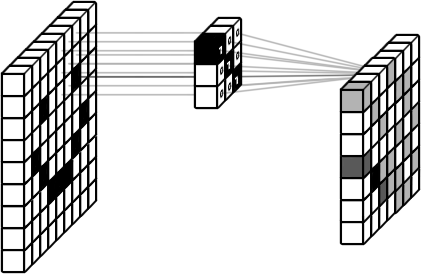
\includegraphics[width=0.5\textwidth]{images/happyConvolution.png}
\caption[Soraya Boza, adapting this image from User Cecbur, \url{https://commons.wikimedia.org/wiki/File:Convolutional_Neural_Network_NeuralNetworkFilter.gif}, with labels added by Jeff Yoshimi.]{A convolutional layer and its components. From left to right: an input image, a 3x3 convolutional filter (which detects edges with a $-45^\circ$ angle), and the resulting feature map. The filter is scanned across the image. At each stage of this scanning process, the dot product of the filter's receptive field in the input image is computed and used to populate the feature map. This whole process is known as a convolution and a layer like this is a convolutional layer.}
\label{cnn_filter}
\end{figure}

\begin{figure}[h]
\centering
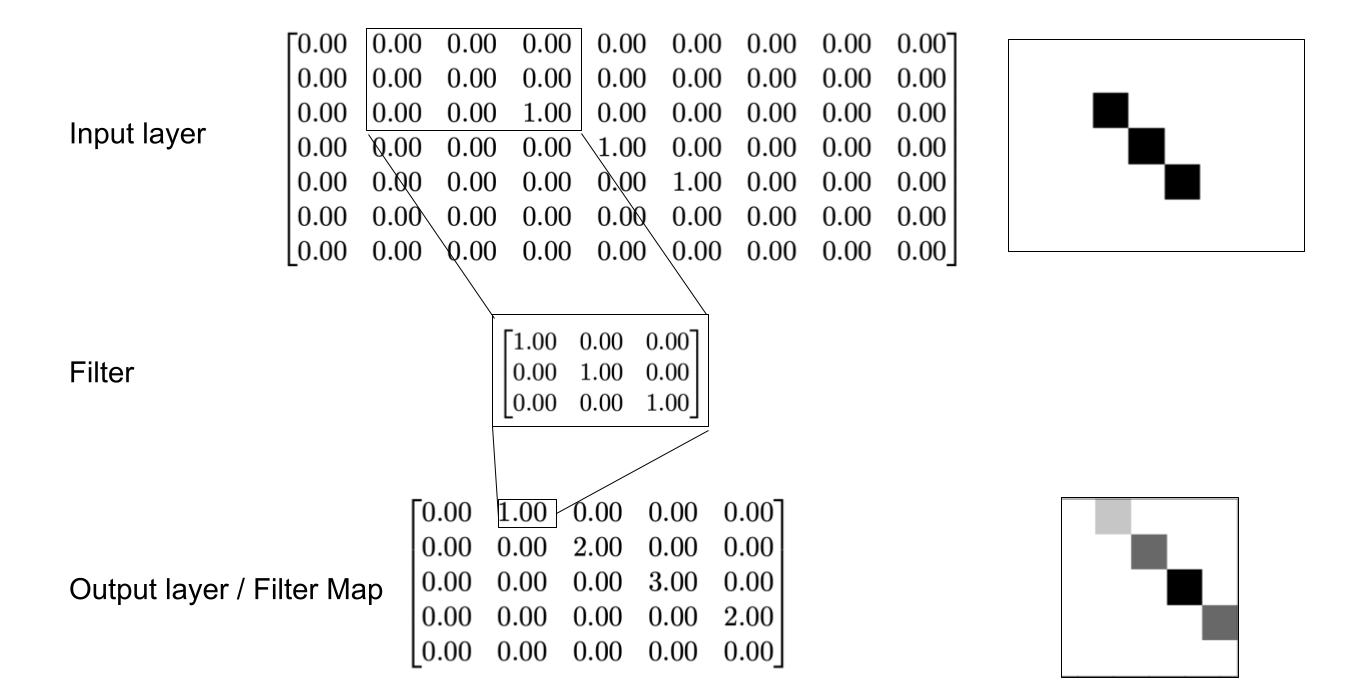
\includegraphics[width=0.7\textwidth]{images/CNN_WorkedExample.png}
\caption[Jeff Yoshimi]{Worked example of a convolutional layer. Notice that the feature map has the highest values where the filter matches the pixel array. In the case shown, the filter matches the pixel array in one pixel only. Imagine the filter sliding over the pixel array, and computing dot products (here: numbers of matching $1$'s), which are used to populate the feature map.}
\label{cnn_workedExample}
\end{figure}

% Expand on weight sharing and add glossary item. Discuss the fact that this is not neurally realistic and ways to understand that.
The weights in a convolutional layer are called a \glossary{filter} or \textbf{kernel}. The weights in a filter are scanned over the source layer to produce outputs. This is a new idea. Rather than a fixed set of weights in a fully-connected weight layer, we have a small set of weights that are reused or shared during the scanning operation (this is also known as ``weight sharing'').

 The source layer of a convolutional layer is often itself a 2d array, prototypically an input image, and so we can think of source layer activations as pixels and the source layer as a pixel array (even when the input is not an image this language is useful). Filters are like small pixel patterns that we slide across the whole pixel array, which ``light up'' most when they are on top of a similar pixel pattern. The filter is generally moved from left to right and top to bottom of the pixel array. At each stage of the scanning operation, it is multiplied by the patch or ``receptive field''  of the pixel array it is on top of.\footnote{To get a better feel for how this works videos are helpful. A good place  to start is with the first animated gif here: \url{https://stanford.edu/~shervine/teaching/cs-230/cheatsheet-convolutional-neural-networks} This video is also great: \url{https://youtu.be/KuXjwB4LzSA}.} The multiplication is a dot product (see chapter \extref{ch_linear_algebra}), where each weight in the filter is multiplied by the corresponding activation of the pixel array, and the results are added together. Recall that the dot product computes something like a similarity score: the more the filter and the pixels match, the greater the dot product will be. The resulting scalar is used to populate one activation in the target layer. Thus, the convolutional layer computes a kind of \emph{sliding dot product} with the source activations, which highlights where the filter matches the pixel array.\footnote{The number of pixels the filter moves at each step is called the \emph{stride}. We are assuming strides of 1 in this chapter (strides can also be different in different directions). One issue that comes up is the edges, which the filter can't be passed over. To handle this, \emph{padding} can be added, in the form of extra zeros around the edges of the pixel array. This page contains an interactive tool that can be used to understand these concepts: \url{https://distill.pub/2019/computing-receptive-fields/}}

% Reference
In practice, convolutional layers operate on a set of matrices  (an input ``volume'') or a batch of these volumes (a 3d or 4d array; see section \extref{sect_tensors}). The output is often also a volume or batch of volumes. How filters work on volumes is discussed below; we start with the simple case where the input and output of the convolutional layer are matrices, which, again, we refer to as a pixel array and feature map.

The idea is illustrated in figures \ref{cnn_filter} and \ref{cnn_workedExample}. A $3 \times 3$ filter is passed over a pixel array, from left to right and top to bottom. At each moment during this scanning process the dot product is computed between the filter and its receptive field in the source matrix (the part of the image the filter is on top of). The output of a convolutional layer is called a \glossary{feature map}. In these examples, the filter is an edge detector, that detects edges at a $-45^\circ$ angle, that is, edges shaped like a backslash `\textbackslash'. In the resulting feature map, notice that the activation is highest when the filter is directly on top of the backslash shape in the happy face, but also produces some activation wherever it is on top of any kind of active pixel. Thus, the feature map gives a sense of where this kind of edge occurs in the input image. The code used to generate figure \ref{cnn_workedExample} is available online, and can be used to edit a small filter and kernel to get a feel for how they produce a feature map.\footnote{See: \url{https://colab.research.google.com/drive/1ywr3z8HRXYNPK-vd34kAATUPVWwwFqQE?usp=sharing}.}

Figure \ref{cnn_filter} illustrates the general idea. Figure \ref{cnn_workedExample} shows an example where all the numbers are included so you can see how the computations are done. Since the input image and the filter are both binary, the dot product simply counts how many places the filter overlaps its receptive field as it is scanned over the image. In the example shown, it overlaps in one place, in the bottom right of the filter.  So that entry in the target layer is populated with a $1$.  Notice that this filter produces the highest value of $3$ only when it is directly on top of the line in the source layer. Try to understand how all the target layer activations are computed. You can also imagine what would happen if the filter or the image were changed.

Again, this is totally different from the weight layers we have been studying throughout the book: there are no fixed connections at all. Instead it is like there is a little floating scanner that gets passed over source layer activations to produce output activations. 

There is a performance advantage to these convolutional layers, thanks to the weight sharing. All that must be trained is (in the example shown in figure \ref{cnn_filter}) $3 \times 3=9$ weights, rather than the $100 \times 100 = 10,000$ weights that would be required in a fully connected dense layer from the input layer to the feature map. This is a huge performance gain and part of what  made it possible with deep learning to train such large networks.

In general, filters--like this edge detector--are not programmed. This is a neural network after all, and neural networks are trained, not programmed (section \extref{intro_comp_nn}), usually using a form of gradient descent (section \extref{sect_gradient_descent}). Networks trained on vision tasks do not need to be told that edge detectors are useful in early stages of processing. They simply emerge as a structure that supports pattern classification when training a network.

\section{Applying a Filter to a Volume}

So far we have considered an artificial example where the input, filter, and feature map were matrices. However, the power of CNNs is that can deal well with more complex tensors. In the context of image processing (and in most applications of convolutional networks), the input is a volume, a set of multiple stacked matrices or channels, a rank 3 tensor or 3d array.  In these cases the filter is really a set of filters (or equivalently, a small 3d array), one ``sub-filter'' (my term) for each input channel. This filter is ``combed'' across the input volume, in the sense that each sub-filter is convolved with a corresponding input channel, and the results are then added together. Figure \ref{combing} gives a sense of how it works. Convince yourself that the shapes make sense.
% Not sure I like this anymore: In a sense this is like a many-to-one connection in a regular neural network. Many nodes connect to one node via a set of weights.  Each weight is multiplied by a different input activation and the results are added up to produce a net input.  Here instead we have a set of sub-filters, each of which is convolved with one channel in an input volume, and the results are added together.: Reference to net input // Show an actual parallel picture of a 3-1 simbrain net. However the analogy breaks down in the many-to-many case.

But the ``combing'' idea is just a way to ease you into the proper way to think of this: as a volume being dotted with a volume. The filter is a little Rubik's cube type object, that gets dotted with an entire receptive field in the input it is passed over. The 27 cuboids in the filter are dotted with 27 components of the input volume, in the way shown in the figure.
% TODO: Add a second image

In general, the depth a filter (the number of channels it has, not to be confused with depth in the sense of number of layers of a network) matches the depth of the input volume. That is, the kernel always ``stretches'' to fit the number of input channels. If not otherwise specified these two values are assumed to match. This is not a necessary feature (filters with fewer channels than the input are possible and sometimes even useful), but it is pretty standard.
% Pierre you mentioned applications with "sculptures" here

\begin{figure}
\centering
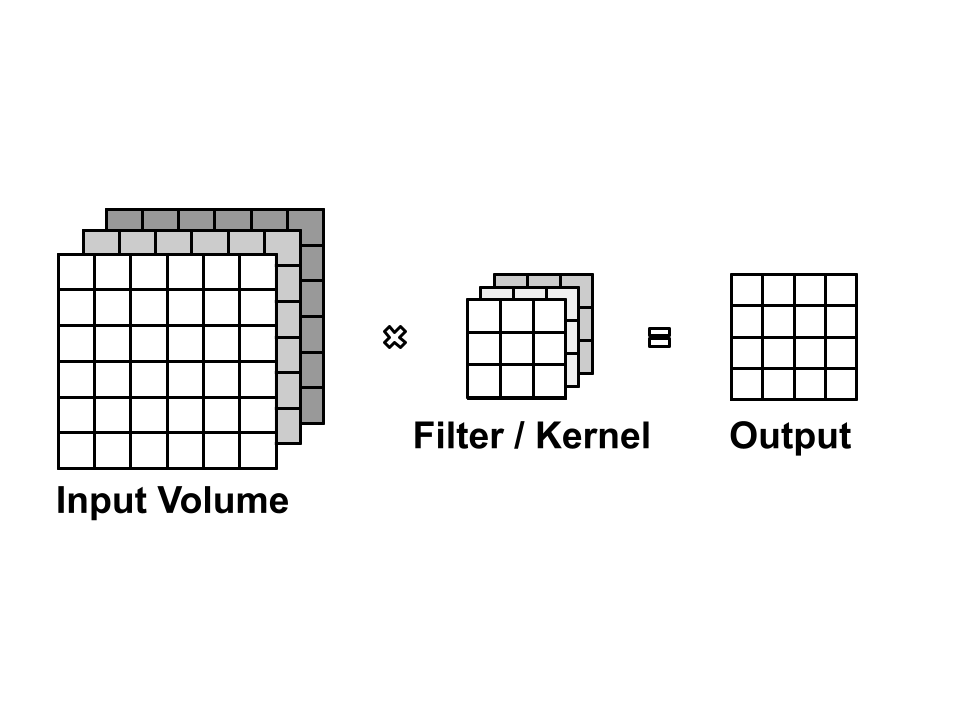
\includegraphics[width=0.5\textwidth]{images/filterComb.png}
\caption[Todo.]{Applying a filter to an input volume. On the left is an input volume, in the middle is a filter (which includes three sub-filters) and on the right is the output volume that results from convolving or ``combing'' the filter over the input. Each sub-filter is convolved with each input channel, and the results are added together at each stage of the convolution. }
\label{combing}
\end{figure}

\section{Filter Banks (Representational Width)}

% More on representational width. Link to transformers and multi-head attention

In general a convolutional layer will involve multiple filters, a filter bank, each of which produces a separate feature map. These generalize the concept of the representational ``width'' of a layer (section \extref{structureNets}) to CNNs. This is part of what gives CNNs their power. Rather than learning just one way to represent inputs, a bank of filters can learn multiple complimentary ways to represent inputs.

% TODO: Keep working and cohering this
 Figure \ref{deep_net2} illustrates the idea. Each filter produces its own output, and the results are concatenated into a new output volume.  Thus the output of a convolutional layer is a set of feature maps. Notice in the image how several of the node layers say ``Feature maps'' plural, or ``F.maps.'' Each feature map in one of these sets is a response to a different filter, for example, edges of different orientation. This is how primary visual cortex reacts to images, so this is a nice model of the brain, hence an example of computational  neuroscience. However, these networks are best known for the engineering benefits, since they are powerful pattern recognition systems.

\begin{figure}
\centering
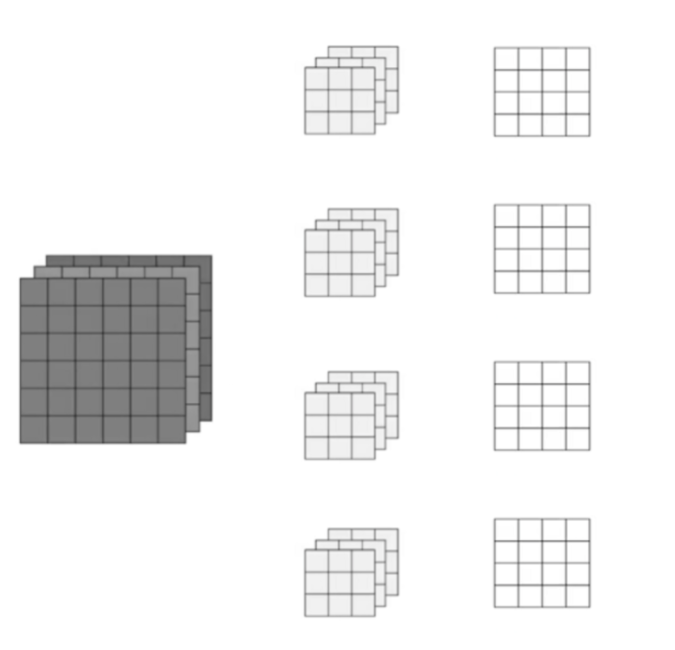
\includegraphics[width=0.5\textwidth]{images/multipleFilters}
\caption[Jeff Yoshimi.]{Result of applying a filter bank to an input volume is an output volume with as many matrices as there are filters in the filter bank. Note that we are here going from a 2x6x6 volume to a 4x4x4 volume.}
\label{combing2}
\end{figure}
% TODO: Change to volume pic and show the concatanated result.

% Need a pass here
These networks develop meaningful representations with training; the representations are not programmed in. This is kind of remarkable to ponder. We did not tell the network we want it to learn to respond to edges. All we focus on in training a network is inputs and outputs, using a labeled data set.  In the case shown in the figure, the training data involve images paired with numbers. The network is given nothing else but these training examples: if you see this picture, it's a 2; this picture is an 8, etc. Then the network adjusts all its parameters (all the weights in its convolutional layers), in such a way as to reduce error.  Edge detectors were learned by training, not programmed in. This is an old connectionist theme. In Nettalk (section \extref{ch_representations}), phonetic categories like consonant and vowel were not programmed in, but emerged with training. With simple recurrent networks  (section \extref{internalRepsRecurrent}), grammatical categories like verb and noun were not programmed in but  emerged with training.

\section{Multiple Convolutional Layers (Depth)}

%TODO: Basic computations needed to think about layer to layer shapes and organize the whole section around the new image

% From Yamins, 2016: "Deep networks through stacking. Since convolutional layer outputs have the same spatial layout as their inputs, output of one layer can be input to another. HCNNs can thus be stacked into deep networks (Fig. 1c). Although the local fields seen by units in a single layer have a fixed, small size, the effective receptive field size relative to the original input increases with succeeding layers. Because of repeated striding, deep HCNNs typically become less retinotopic with each succeeding layer, consistent with empirical observations4."

% Compositional or layered complexity.  Example: the first layer of filters captures patterns like edges, corners, dots etc. Subsequent layers combine those patterns to make bigger patterns (like combining edges to make squares, circles, etc.). Now as we move forward in the layers, the patterns get more complex; hence there are larger combinations of patterns to capture. That's why we increase the filter size in subsequent layers to capture as many combinations as possible.

In a full deep network many convolutional layers and dense (fully-connected) weight layers are combined, sometimes as many as 100 or more! This allows the network to learn to identify not just simple features like edges or curves, but also \emph{features of features}, like combinations of curves which make more complex shapes, and then combinations of these shapes. 
% More here; put the Selfridge reference here

\subsection{Pooling}

% Not a convolutional layer, but very rarely used unless it is a CNN.  So it makes sense here. Not used in transformers, or LSTM. Use for things that are getting bigger and bigger so they must go down a good. Also good because they can be used for variable sizes.
% Usually looks at just one filter? 

In a many-layered set up, other layers besides convolutional layers are used. As can be seen in figure \ref{deep_net2}, there are other kinds of layers besides convolutional layers which are nonetheless similar in terms of how they work. They also involve scanning a small window over an input matrix or volume, and applying an operation at each stage of the process. There are two common cases here:

\begin{description}
\item[Max pooling] In each window, the maximum number is taken and written to an output matrix.
\item[Average pooling] The average value across a window is written to an output matrix.
\end{description}

These are sometimes called pooling, subsampling or downsampling methods. They are valuable in that they reduce the overall size of the network while preserving important structures.

% TODO: Double check below and of course, find a better picture or make one!
In applying these layers the number of channels should not change. The pooling or subsampling is done separately on each matrix in a volume, and produces a corresponding new volume with the same number of matrices, where each matrix has a smaller size. One unfortunate feature of figure \ref{deep_net2} is that it obscures this fact. Between subsampled layers we should have smaller matrices (as is shown) but the same number of matrices (which is not shown).

% TODO: Redo
\begin{figure}[h]
\centering
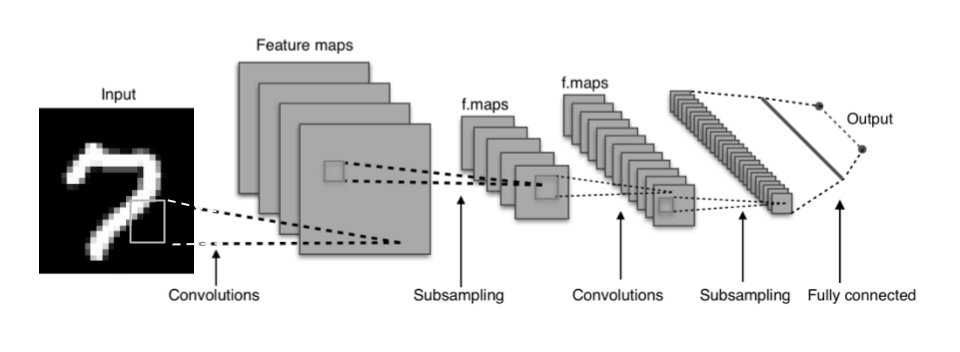
\includegraphics[scale=.45]{./images/deepNet.png}
\caption[Adapted from a creative commons image by Aphex34 at \url{https://commons.wikimedia.org/wiki/File:Typical_cnn.png} ]{A deep neural network, trained to recognize images. The convolutional layers scan over the inputs they are linked to. The filters are not shown in this picture, only the input volume and hidden layer volumes and final node layers. }
\label{deep_net2}
\end{figure}

\subsection{Dense Layers and Flattening}

% Glossary for flatten and break it out

The final layers of a deep network are often more conventional fully-connected dense layers. The idea is to start with layers that learn these complex features, then to compress these representations with subsampling, and finally to present the results to the final layers, which are basically familiar backprop networks presented with the results of a whole lot of convolving and subsampling. Between the convolutional and pooling layers which are often 3d arrays, a flattening layer must be introduced to change the format to that of a traditional neural network.

\section{Applications of Deep Learning}

% This section obviously needs to be developed
% What do convolutional layers correspond to in the brain?
 
As discussed in section \extref{deep_revolution}, deep networks and deep learning led to a revolution in neural networks beginning in the 2010s. The revolution was in engineering initially, but the history of deep networks shows that they have applications across all the domains of neural network research: engineering, computational neuroscience, connectionism, and computational cognitive neuroscience. 

Deep network models originate in  computational neuroscience models of vision that were developed in the 1970s and 1980s \cite{fukushima1982neocognitron}.  These ideas were later used to engineer pattern recognition networks. A famous early application was recognizing zip codes written on envelopes \cite{lecun1989backpropagation}. As deep networks became mainstream based on technical improvements (big data, GPU and hardware acceleration, better architectures and training algorithms), scientists began using them, for example, to model the response profile of neurons in the visual system (recall the discussion of figure \extref{deepLearning_Vision} in chapter \extref{ch_neuro}). 

The idea is also relevant to connectionism and computational cognitive neuroscience. Recall from the history chapter that the concept of layered feature detection goes back to Oliver Selfridge and his ``pandemonium'' model, which at the time just speculated that in seeing letters a hierarchy of ``demons'' pass messages along: from edge demons to curve edges and finally to the output layer's ``B demon'' (see figure \extref{selfridge} in chapter \extref{ch_history}). Deep networks instantiate this idea, in such a way that we can actually  see what their receptive fields are.\footnote{The receptive fields can be quite strange and even disturbing. See \url{https://distill.pub/2017/feature-visualization/} for some striking demonstrations.}  The significance of these networks for psychology is still in its infancy, but early results are promising \cite{zorzi2013modeling, ritter2017cognitive}.
% Work more on interpreting what is happening in that distll article, and add some material here, including pictures of the weird features. Then add some colab demos to the course.
